\subsection{Program master GBTx with external \itwoc adapter}
As said in the previous section, the master GBTx board must be programmed via an
external \itwoc adapter first.
A Windows 7 computer on the rack is used. The GBTx programmer is located at:

\begin{minted}[frame=single]{powershell}
DT_Rack\GBTx_programmer\GBTxProgrammer.jar
\end{minted}

\begin{figure}[ht]
    \centering
    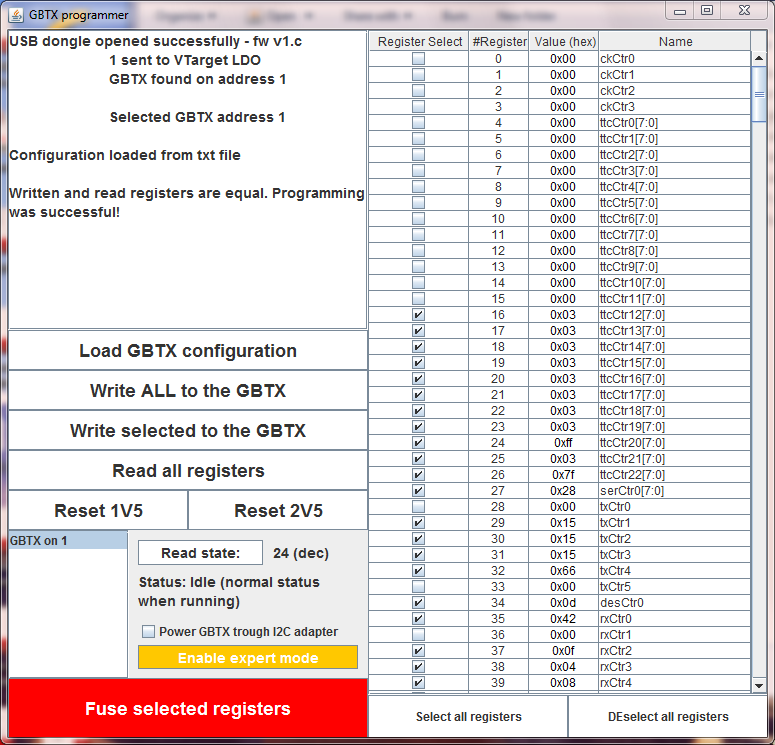
\includegraphics[width=0.9\textwidth]{res/gbtx_programmer_v1_ui.png}
    \caption{A typical UI for GBTx programmer.}
    \label{fig:gbtx-programmer-ui}
\end{figure}

Launch the programmer, a typical UI is shown in
\autoref{fig:gbtx-programmer-ui},
Click ``Load GBTX configuration'' and load a configuration file.
The configuration file is located at:

\begin{minted}[frame=single]{powershell}
DT_Rack\GBTx_programmer\GBTx_TRx_v12_test_withWatchDog.txt
\end{minted}

Then click ``Write ALL to the GBTX''. Check the returned message to make sure
everything works (supposedly).
Now click ``Read state''.
If the master GBTx is configured corrected and is connected to a working
MiniDAQ, the return value should be:

\begin{minted}[frame=single]{powershell}
24 (dec): Idle (normal status when running)
\end{minted}
